% !TeX root = ../main.tex
% Add the above to each chapter to make compiling the PDF easier in some editors.

\chapter{Background}\label{chapter:background}

\section{Intel SGX}
The Intel Software Guard Extension (Intel SGX) is an instruction set available for Intel Core CPUs since the 6th generation in 2015. 
It allows software developers to create programs that are run inside so called “enclaves”, i.e. trusted execution environments to protect programs, including their secret values from other processes. To ensure this, special memory management mechanisms, enclave control structures and new atomic CPU operations have been implemented. 
This chapter will explain the most important aspects of Intel SGX. A more detailed examination of the components can be found here: \cite{sgx_explained}, \cite{sgx_101}, \cite{sgx_developer_guide}.\\

\textbf{1. Physical Memory:}\\
To ensure that data within an enclave is protected from outside access, Intel SGX uses a special memory region, called Processor Reserved Memory (PRM). It is a subset of the DRAM but not accessible by other operating system software, such as the hypervisor or the kernel. The CPU even protects it from DMA accesses by other hardware devices.
All the data of an enclave, including the Code, is stored in the Enclave Page Cache (EPC), i.e. a subset of the PRM, consisting of 4 KB pages which can be assigned to an enclave via normal system management software. However, since this software is not trusted according to Intel's Threat model, memory allocations and the state of the EPC are stored in the Enclave Page Cache Metadata (EPCM). This data-array has one entry per EPC page. This entry helps the CPU efficiently identify the owning enclave of a page and ensures that one EPC page is only assigned to one enclave.\\

\textbf{2. Virtual Memory:}\\
The virtual memory of an enclave contains a designated memory region, called the enclave linear address range (ELRANGE), which only maps to the secure EPC region in physical DRAM. \cite{sgx_101} To protect against possible address translation attacks, the virtual address of a EPC page is stored inside the corresponding EPCM entry of that page, after it has been allocated. With the help of this information, the CPU can determine during a translation process from virtual to physical address whether the virtual address matches the value in the EPCM entry and therefore check that ELRANGE addresses are only mapped to EPC pages. It is also possible to set special rwx-permissions in the EPCM, which are also checked by the processor. \\

\textbf{3. Data Structures:}\\


Another important component to SGX are Thread Control Structures (TCS). They are stored in a dedicated EPC page, with similar access restrictions like SECS and define the context switches between non-enclave and enclave code. For a multithreading environment, each logical core that executes enclave-code, has a separate TCS. \\

\textbf{4. Interrupt and Exception Handling:}\\
Unexpected interrupts often pose a security threat, since sensitive data used for computations in the program still resides unencrypted inside the registers, during the execution of exception routines. 
As a countermeasure to this problem Intel integrated the State Save Area (SSA). This area is used to store the enclaves thread execution context (a set of general-purpose registers and the XSAVE instruction) while an exception is handled. Each TCS references a contiguous sequence of EPC pages which form the SSAs. So once an interrupt is triggered, the CPU immediately transfers the content of the registers to the SSA pages and clears the registers. The pages are marked as regular EPC pages in the EPCM to allow the exception handler of the enclave to access the information if required. \cite{sgx_101}  \\

\textbf{5. Enclave Lifecylce:}\\
Intel SGX provides a set of CPU instructions to manage the life cycle of an enclave. These management instructions can only be executed by the system software. The state diagram in Figure \ref{enclave_lifecycle} shows the different state transitions during the creation and execution of an enclave. 

The first step to create an enclave is the ECREATE instruction. It fills an empty, unassigned EPC page with the contents of a predefined SECS structure from untrusted memory, verifies this data and sets the SECS INIT attribute to false, which prevents the enclave from executing yet. Now the EADD instruction can be used to load initial data and code into the EPC, creating TCS pages and regular pages. Note that it is only possible to allocate EPC pages to an enclave when the SECS is marked uninitialized, otherwise a \#GP fault will be triggered. Moreover, during the loading stage, the CPU will create a cryptographic hash of the initial data, which will become the enclave’s measurement hash after initialization, which is of very important to the remote attestation process. This value in the MRENCLAVE measurement register of the SECS can be updated with the EEXTEND instruction. 

Before calling the EINIT instruction to initialize an enclave, the system software has to use a high privileged, Intel authored Launch Enclave to retrieve a special token structure. Only with this input the EINIT instruction is able to set the INIT attribute in the SECS to initialized.\cite{sgx_explained}
By calling the EENTER instruction the enclave can then finally start executing user code. 

\begin{figure}
	\begin{center} 
		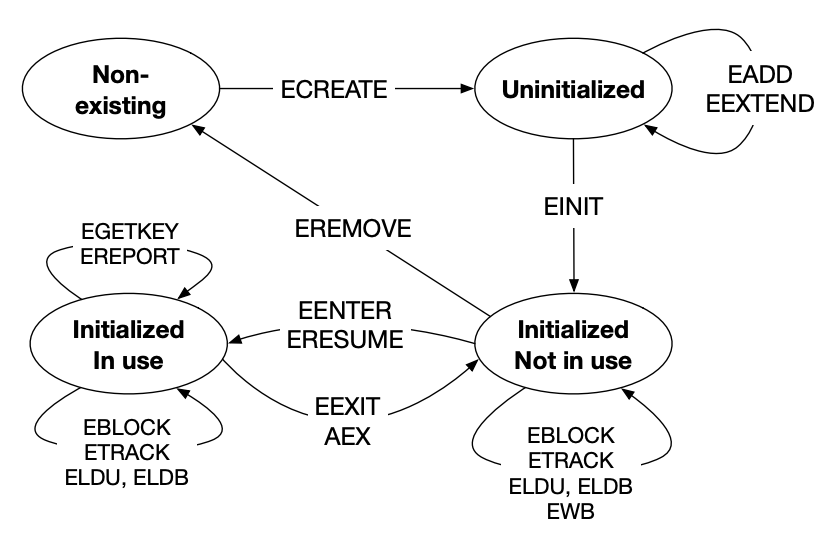
\includegraphics[width=0.7\linewidth]{figures/enclave-life-cycle.png}
	\end{center}
	\caption{SGX enclave life cycle management instructions \cite{sgx_explained}} 
	\label{enclave_lifecycle}
\end{figure}

\section{Remote Attestation}
Remote Attestation is the process of authenticating the hardware and software components of a remote system, with the goal to increase the trustworthiness of a system. The challenger sends a request to the remote system to generate an attesation report for the Trusted Execution Environment, that he owns. The attestation prover then collects measurements about the software stack of the isolated TEE and it’s configuration and combines and signs them in an attestation report. This report is then sent, ideally over a secure connection, to the relying party, which forwards the report to an internal verification service. The verification service then compares the measurements and configuration settings against a set of expected values and a policy, verifies the signature chains and decides whether to trust the server or not. This general remote attesation flow is depicted in figure \ref{general_attestation_flow}.

\begin{figure}
	\begin{center} 
		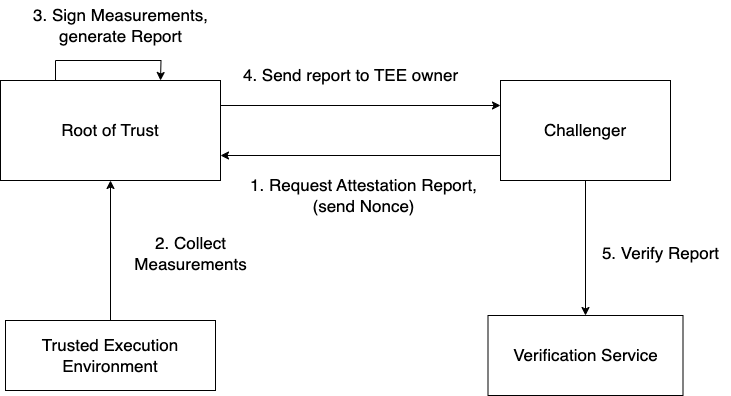
\includegraphics[width=0.7\linewidth]{figures/general-attestation-flow.png}
	\end{center}
	\caption{General remote attestation flow (simplified)} 
	\label{general_attestation_flow}
\end{figure}

Establishing trust in the measurements inside an attestation report without trusting the system requires a \textit{root of trust}. In case of confidential computing technologies the root of trust is the secure hardware, e.g. the AMD Secure Processor or the Intel SGX CPU. The measurements generated by these components are signed through a certificate chain by the \textit{trust anchor}, i.e the AMD root CA or Intel root CA, which guarantees the trustworthiness of the attestation report. 

The fundamental process of collecting measurements, creating and signing attestation reports, etc., remains largely consistent across different confidential computing technologies. However, significant variations exist in the implementation details and the structure and data of the generated attestation reports. Consequently, the integration of a custom remote attestation service necessitates a thorough analysis of the specific technologies employed.
The subsequent chapter will therefore introduce the core concepts of Intels third party remote attestation mechanism. 

\section{Intel SGX DCAP}
Intel offers two different types of remote attestation: 

\begin{enumerate}
	\item Intel Enhanced Privacy ID (EPID) Attestation
	\item Elliptic Curve Digital Signature Algorithm (ECDSA) Attestation via the SGX Data Center Attestation Primitives (DCAP). 
\end{enumerate}

EPID provides attestation with increased privacy protection features based on the Intel SGX platform software. It is available on specific Intel Core, XEON E and XEON E3 processors, requires the relying party to have internet access for connecting with the Intel managed attestation service and is therefore mainly used on client machines. \cite{sgx_website}

DCAP Attestation on the other hand was designed for providers to build their own third-party attestation service. It is available on specific Intel XEON scalable and XEON E3 processors and requires a specific SGX feature called Flexible Launch Control (FLC). FLC mainly enables platform owners to choose an arbitrary Launch Enclave which generates the enclave launch tokens. It is also important to note that this feature must be supported by the BIOS as well. \cite{sgx_website}
Since DCAP requires more provider managed infrastructure than the EPID based attestation, it offers more control and flexibility of the attesation and report generation process. 

To generate an attestation report (a quote) for an SGX enclave, the following steps have to be performed (see figure \ref{dcap-quote-generation}): 

First, the challenger makes a call to the application on the untrusted system to request a report (step 1).
In turn the Application calls the Enclave to generate a report (step 2).
Using the EREPORT instruction the CPU creates a report including the measurements and sends it back (step 3). Since the enclave report is not signed yet, the user application makes a call to the Quoting Enclave (QE) in step 4 to verify the report and to add a cryptographic signature. The Quoting Enclave thereby communicates with Provisioning Enclave (step 5), which is used to sign the QE report with the platform specific Provisioning Certification Key (PCK) and to add the appropriate certificate chain. The Provisioning Enclave retrieves Certificates from the Intel Provisioning Certification Service (PCS) or the local Provisioning Certification Caching Service (PCCS) to speed up performance in step 6 and 7. After the Provisioning Enclave finished, it returns the report back to the QE, which signs the report with the attestation key, that is generated inside the QE (step 8 and 9) and returns the signed report (quote) to the application. This data is then ideally transferred over a secure channel to the client machine for verification (steps 10 and 11).  \cite{gramine_dcap_attesation}


\begin{figure}
	\begin{center} 
		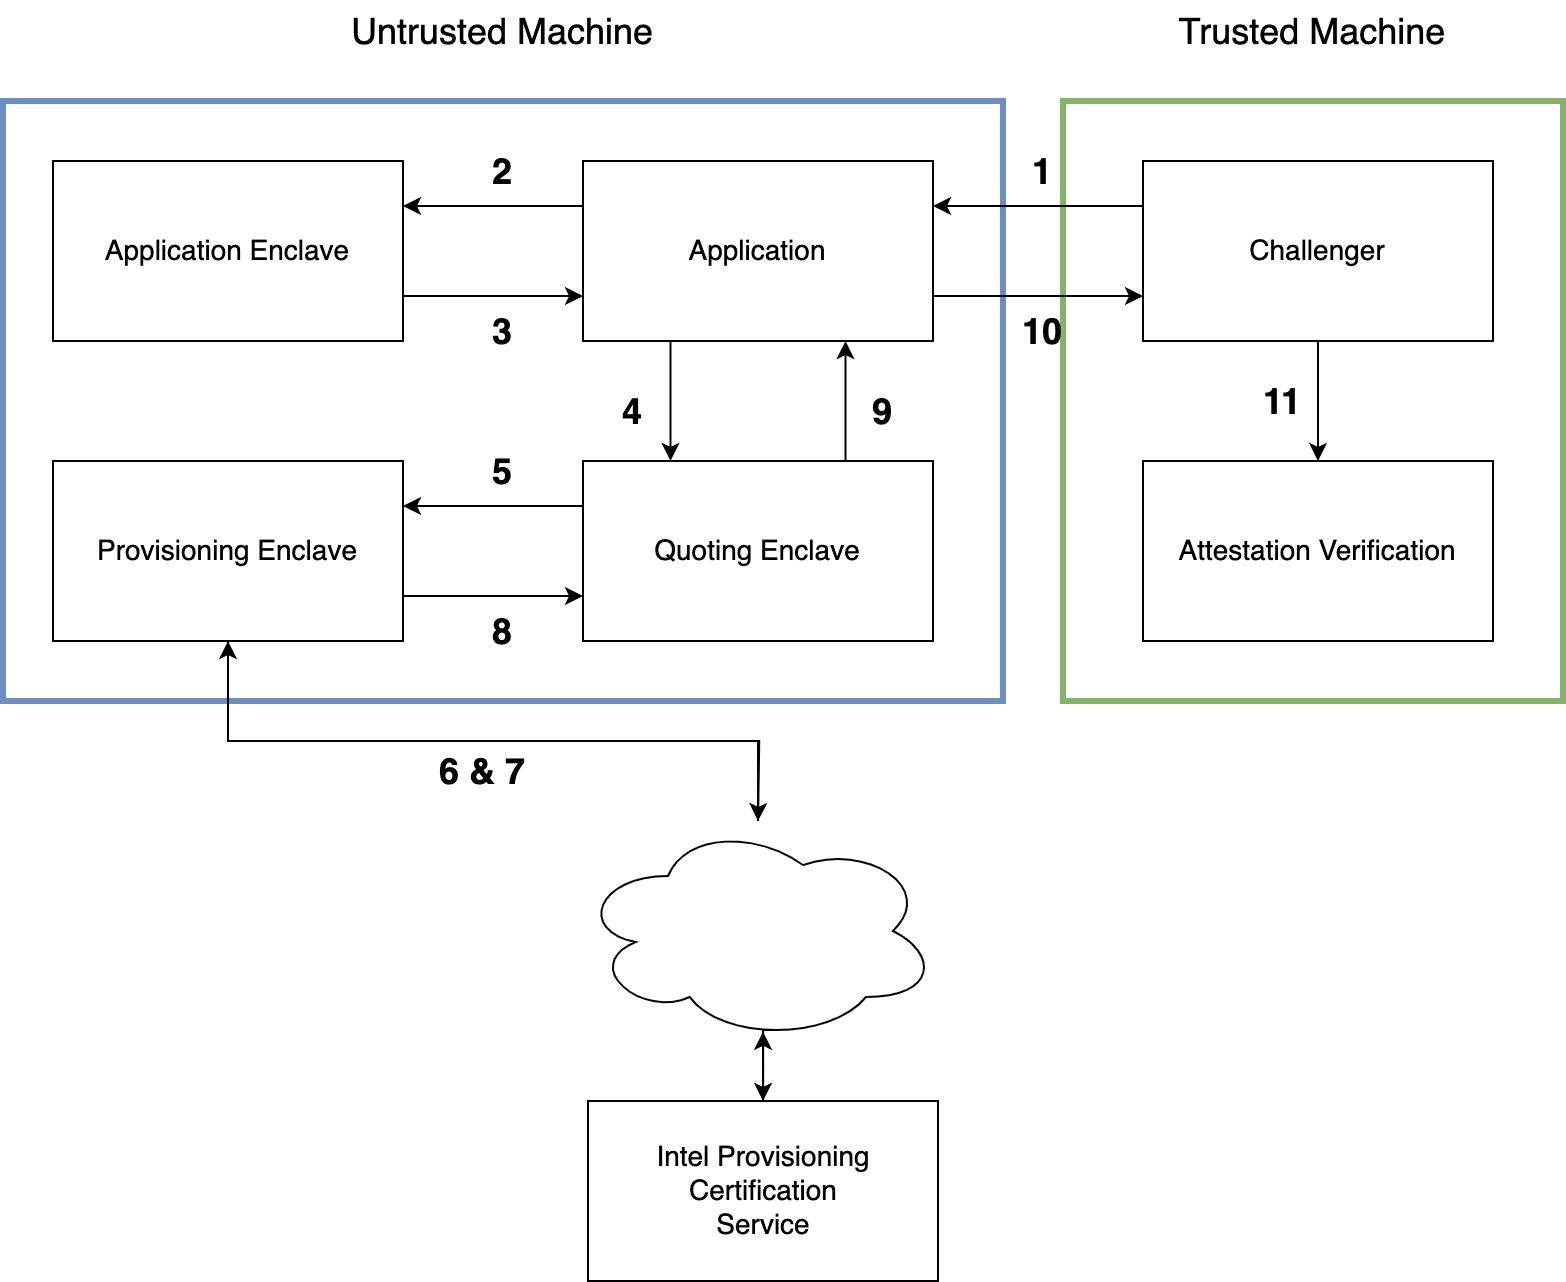
\includegraphics[width=0.7\linewidth]{figures/dcap.drawio.png}
	\end{center}
	\caption{DCAP based remote attestation flow \cite{dcap_quote_generation}} 
	\label{dcap-quote-generation}
\end{figure}

The Intel SGX certificate hierarchy is shown in figure \ref{sgx-cert-hierarchy}. The root of trust is the Intel SGX Root CA certificate. This Certificate signs several Intermediate certificates: The Intel SGX PCK Platform/Processor CA Certificates, the Intel SGX Root CA Certificate Revocation List (CRL) and the Intel SGX TCB Signing Certificate. Depending on the platform, either the PCK Platform CA Certficate or the Processor CA Certificate is used to sign the leaf PCK Certificate and revocation list for the unique PCK key. This key is issued by Intel during manufacturing and rooted to the CPU hardware fuses. The TCB Signing Certificate on the other hand is used to Sign the TCB Info, QE Identity and Quote Verification Enclave (QvE) Identity data structures which are used to verify a quote. As stated earlier all this data is available through an API from Intels Provisioning Certification Service and then stored inside the Provisioning Certification Caching Service (PCCS) on the platform. Certificates, revocation lists and other collateral data inside the PCCS is automatically updated regularly so a newly signed quote contains the latest information. 

More information about the implementation specifics of ECDSA based quote generation and verification with DCAP can be found in chapter \ref{chapter:integration}. 

\begin{figure}
	\begin{center} 
		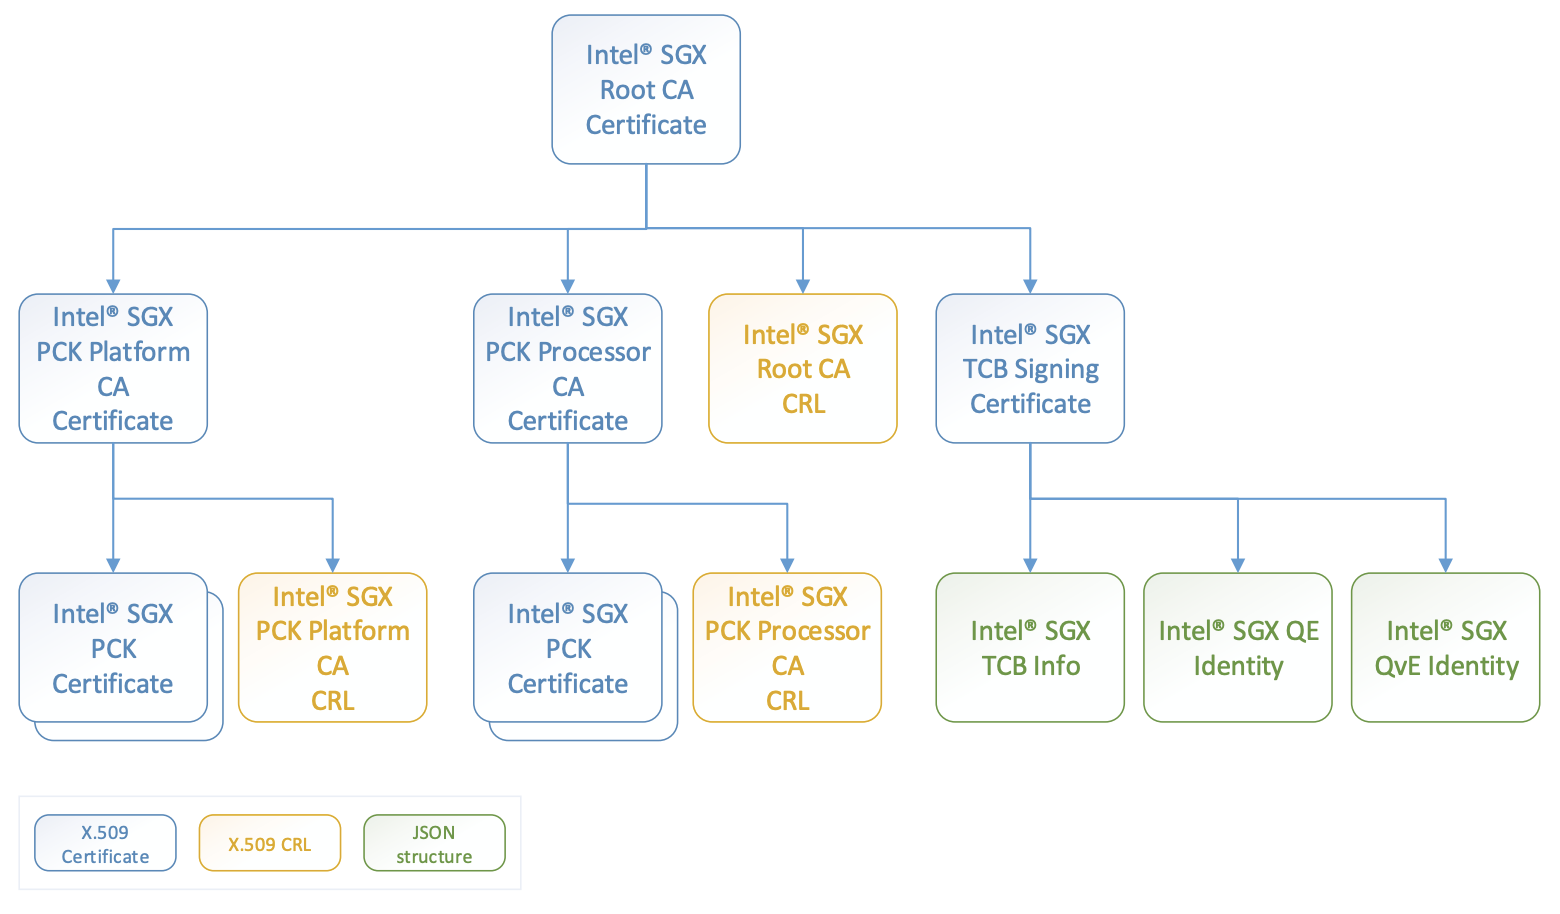
\includegraphics[width=1.0\linewidth]{figures/sgx-cert-hierarchy.png}
	\end{center}
	\caption{Intel® SGX ECDSA Public Key and Data Structure Hierarchy \cite{pccs_design_guide}} 
	\label{sgx-cert-hierarchy}
\end{figure}

\section{CMC Framework}
The Connector Measurer Component (CMC) is a Universal Remote Attestation Framework developed by the Fraunhofer AISEC Institute. More precisely, it provides tools and software to enable remote attestation of computing platforms, as well as remote attested TLS channels between those platforms for secure communication. It is was written in Go (golang) and currently supports attestation for Trusted Platform Modules (TPMs), AMDs Secure Encrypted Virtualization Technology (SEV-SNP) and ARMs Platform Security Architecture (PSA). 

The main component of the framework is the cmcd daemon. It acts both as an attestation prover and verifier. As a prover within the TEE on server-side, it is used for the assembly of a comprehensive attestation report structure. The collected attestation evidence (the protected measurements) from the hardware trust anchor are hereby combined with additional metadata about the device and the software. Additionally, the verifier chooses a nonce, which is also included in the measurements for freshness and replay protection. 
Therefore as a verifier it can perform the attestation solely given the report and a list of trusted CAs specified by the verifier owner. It has to verify the corresponding signatures and certificate chains of the measurements and the metadata and compare the values. If all checks pass, including optional policies defined by the verifier owner, the system is successfully attested. 

\begin{figure}
	\begin{center} 
		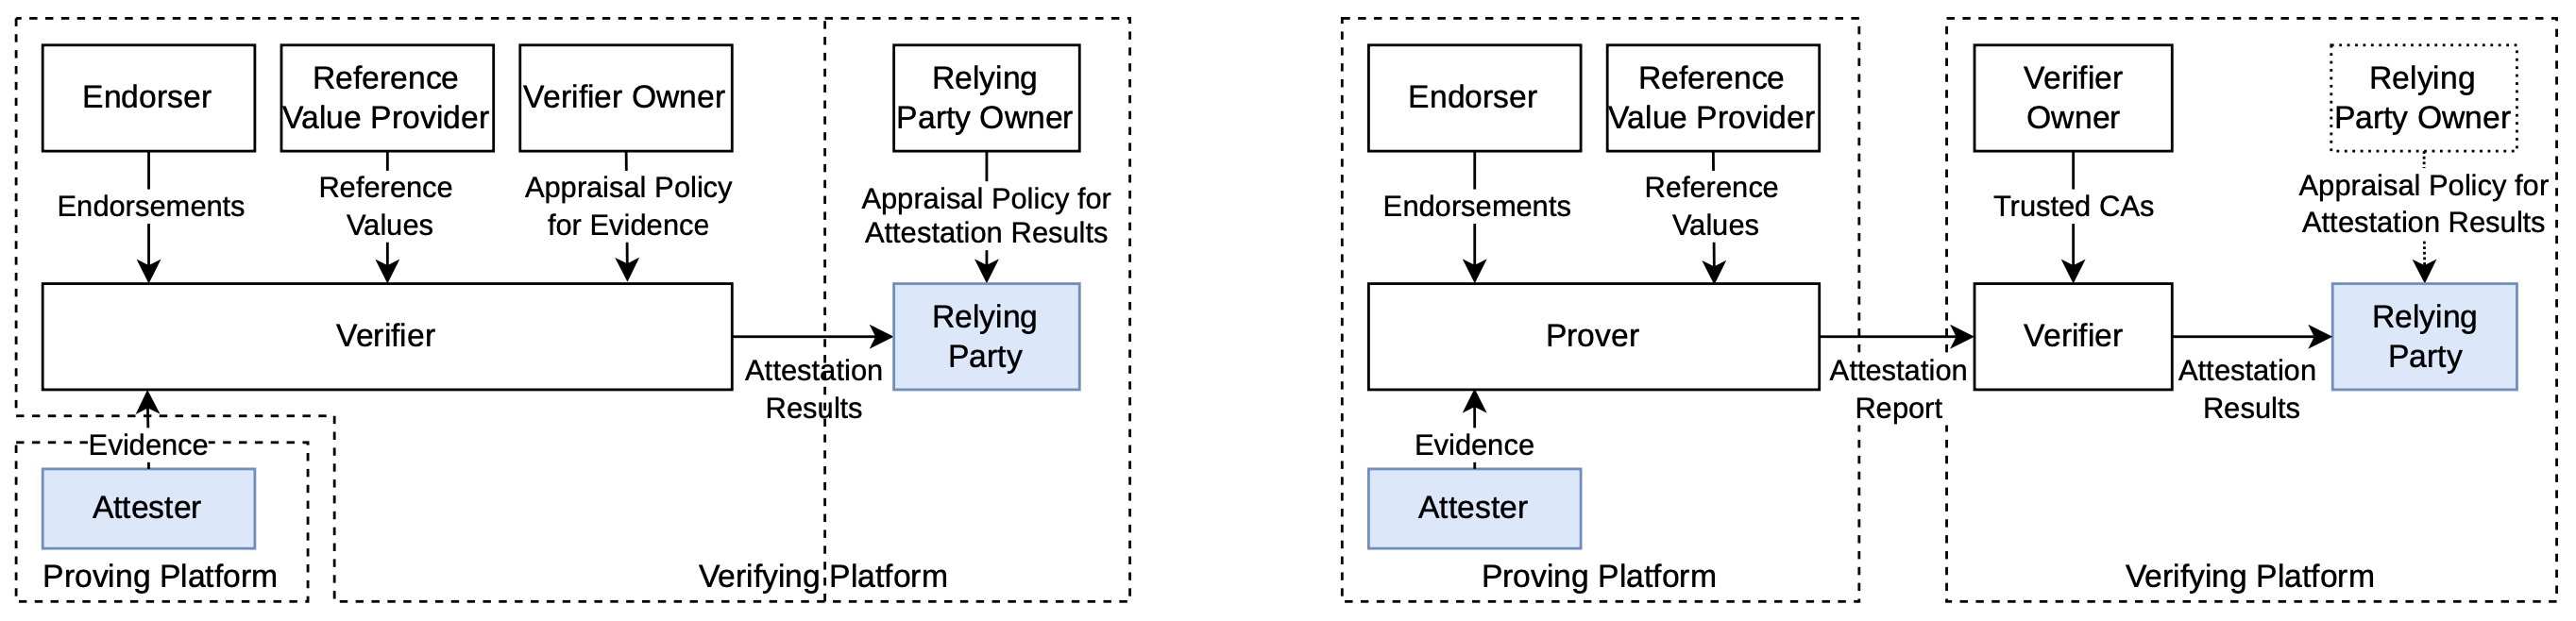
\includegraphics[width=1.0\linewidth]{figures/rats-vs-cmc.png}
	\end{center}
	\caption{Generic RATS architecture (left) and CMC framework (right) \cite{CMC_paper}} 
	\label{rats-cmc}
\end{figure}

Unlike other generic architectures, such as Remote Attestation Procedures (RATS) defined in RFC 9334, this approach shifts the responsibility of providing meaningful metadata to the prover instead of the verifier. 
This has two main advantages. Firstly, it reduces the number of dependencies of the relying party and the verifier, thus simplifying complexity of the verifier. Secondly, as the prover posesses real-time access to updated information about the platform's software stack, it is considerably easier to generate valid information. The respectives architectures can be seen in figure \ref{rats-cmc}.

Since both the attestation reports and the metadata are generated and structured differently on the respective platforms, the generic measurement and signer interfaces were created in the attestation report package, which can be called by cmcd. The actual implementation of these interfaces can be found in the corresponding drivers for the specific Confidential Computing technologies, e.g. snpdriver, tpmdriver, etc. (see figure \ref{cmc-arch}).

During the provisioning process, the cmcd interacts with an Enrollment over Secure Transport (EST)-based provisioning server, called provserver, which serves multiple roles. It issues certificates for software signing, executes TPM Credential Activation and facilitates the provisioning of certificates and metadata. For the purpose of demonstration, the server was deliberately designed with simplicity in mind. In real-world scenarios on the other hand, its functionalities may be distributed across distinct servers, such as a CA server and an internal metadata server. \cite{Github_CMC}

Suppose there is a SEV VM operating on a remote server. The CMC framework is installed once on the remote cloud server to generate and transmit attestation reports. Additionally, the CMC is installed once on the client side to verify these reports. Multiple communication interfaces are available for applications to interact with the CMCD. These interfaces include a socket API, gRPC, and Constrained Application Protocol (CoAP). The purpose of these interfaces is to enable attestation for services operating with restricted hardware access, such as within a container (refer to figure \ref{cmc-arch}).
To ensure that the data is also protected during transmission and to prevent Man-in-the-middle attacks, the cmc offers a library for TLS channel binding (aTLS). It implements a trusted channel protocol based on top of TLS to bind the attestation evidence to the secure channel endpoint, which is used to communicate with the attested device. \cite{CMC_paper}
According to \cite{trusted_socket_layers}, Channel binding refers to the process of ensuring the absence of a MITM between two authenticated endpoints within an inner protocol, while utilizing a secure channel from an outer protocol. The standard approach thereby is to generate a unique identifier, called channel bindings, for the outer protocol and to bind this identifier to the run of the inner protocol.  

\begin{figure}
	\begin{center} 
		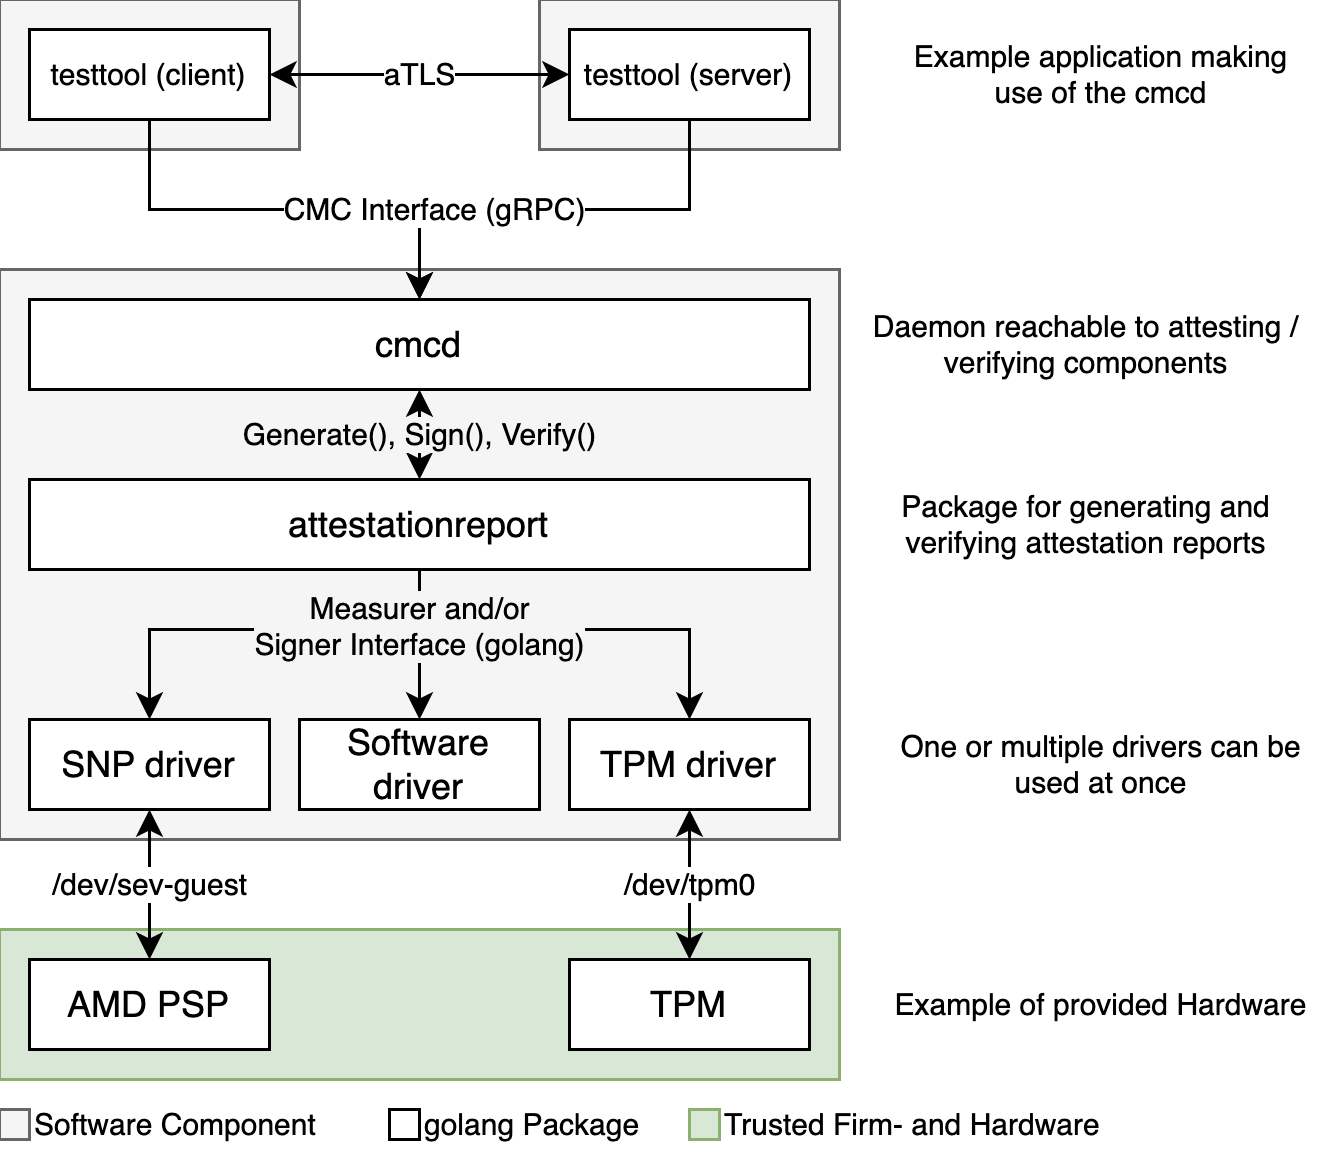
\includegraphics[width=0.6\linewidth]{figures/cmc-arch.png}
	\end{center}
	\caption{CMC architecture overview \cite{CMC_architecture}} 
	\label{cmc-arch}
\end{figure}
